 \section{Evaluation}
 \label{sec:eval}

%  \wajih{Be consistent with datasets in each research question. Sometimes you use OpTC and sometimes you use E3 and you don't even explain why you excluded the other datasets. Rule of thumb is use all the datasets for the experiments unless you have reason or justification why you excluded certain datasets.}

 %\mati{Evaluation section has some writing inconsistencies. I will make a pass over it later today to fix it.}

%  \wajih{the word DISTDET is not consistent in the paper.}

 %\wajih{Use macros for common words in this whole section.}

 %\wajih{Be consistent with the terminology that you used in the abstract/intro.}

 %\wajih{Captions need to be lowercase}



%We evaluate \Sys using the open-source datasets \darpa E3 and \optc, which comprise system audit logs that simulate enterprise environments. These logs are collected from both Windows and Linux operating systems.



%\wajih{We also need to handle as ORTHRUS in the related work or evaluation section. I would love to hear creative way we can handle that.}

%\wajih{Handle this comment in the evaluation section: "I'm quite concerned about the evaluation results in Table 2. It doesn't look right to me that the number of malicious nodes in DARPA TC datasets can be sometimes around 20\%!"}

%\wajih{ We claim that the categorization-based ensemble improves convergence. But there is no empirical convergence analysis in the evaluation section e.g., training loss curves or number of FL rounds, etc. }

%\wajih{Add in the evaluation section how many clients we have in each dataset. "I can't find the number of FL clients in your text" }

Our evaluation experiments are conducted on a machine running Ubuntu 18.04.6 LTS, equipped with a 10-core Intel CPU, NVIDIA RTX 2080 GPU, and 120 GB of memory. In our experiments, we set the federated learning rounds and the number of categorized \gnnshort to 10 per host. Each model is trained for 20 epochs per round. We use regularization and dropout layers in our models to avoid overfitting. To evaluate \Sys, we address the following research questions: %\wajih{I have moved things around so align the RQs with that.}

%\wajih{RQ6 is not in this section. so please remove it. }

%\wajih{Add section references like I added for RQ1}

% \Fix{There are eight subsection in the evaluation while we have six research question. Make them consistent. This can confuse reader. Also, if you moved something to Appendix, refer them below. }

% \wajih{These are just too many research question. You need to combine similar RQs into one. If you think something is an ablation study then move it to the ablation study section. }
\begin{itemize}[leftmargin=*,itemsep=0.1em, parsep=0em, topsep=0em]
  \item \textbf{RQ1.} How does \Sys compare to vanilla privacy-preserving \pids in terms of detection performance? (Section~\ref{sub:detect:perf:vanilla})
  \item \textbf{RQ2.} How does \Sys compare to existing systems in terms of detection performance? (Section~\ref{sub:detect:perf})
  \item \textbf{RQ3.} How scalable is \Sys in an enterprise-level setting with multiple host machines? (Section~\ref{cost_metric})
  \item \textbf{RQ4.} How robust is \Sys against various adversarial attacks?
  %\item \textbf{RQ5.} How effective is the Word2vec harmonization scheme for handling feature heterogeneity? (Appendix~\ref{sub:word2vec:harmonization:efficacy})
  %\item \textbf{RQ6.} How effective is the categorization-based \gnnshort ensemble for handling data heterogeneity? (Appendix~\ref{sub:categorized:learning:efficacy})
  \item \textbf{RQ5.} How does \Sys compare to existing FL solutions in addressing data heterogeneity and non-IID challenges? (Appendix~\ref{sec:fedalternatives})
  % \item \textbf{RQ6.} How robust is \Sys against adversarial mimicry attacks?
  \item \textbf{RQ6.} What is the resource consumption of various components of \Sys and its end-to-end processing time on a client machine? (Appendix~\ref{sec:resource_consumption})
  \item \textbf{RQ7.} What does the ablation study reveal about \Sys's effectiveness across key factors like \gnnshort submodels, averaging rounds, federated averaging rounds, \wordvec harmonization and categorization-based \gnnshort ensemble? (Appendix~\ref{app:ablation})
  
  \end{itemize}  


\PP{Implementation} \Sys is developed in Python with around 5500 lines of code. It leverages the PyTorch and Torch Geometric libraries to implement the federated provenance graph learning framework. The graph learning framework uses the GraphSAGE~\cite{hamilton2017inductive} family of \gnnshort. Our architecture consists of two graph convolution layers with a Tanh activation function in between. The last layer uses a softmax function to output class probabilities for the nodes. For implementing the \wordvec model, we employ the Gensim library. Secure communication between clients and the utility server is ensured through Python's Cryptography module. The federated averaging, semantic vector harmonization, and entity categorization modules are implemented as individual Python functions on the central and utility servers.

% \PP{Datasets} We have utilized the \darpa E3~\cite{error3}, E5~\cite{bug5}, and \optc~\cite{darpaoptc} datasets for our evaluation. The E3 and E5 datasets consist of several adversarial engagements that simulate real-world APTs on enterprise networks. In these exercises, the red team aims to exploit vulnerabilities in the enterprise's services while hiding their attacks behind benign system activities. The logs captured from these exercises are documented under various scenario names, including Cadets, Trace, Theia and ClearScope. The \optc dataset, another open-source resource from \darpa, encompasses a comprehensive collection of audit logs from an enterprise environment with 1,000 hosts. This dataset includes six days of benign system logs, serving as training data for our system to learn normal behavior patterns. Subsequently, attack logs span three days of system activities, featuring red team tactics such as initial compromises, privilege escalations, malicious software installations, and data exfiltration. Each of these datasets is accompanied by ground truth documents that facilitate the distinction between benign and malicious events. For our evaluation, we employ attack labels from existing systems, such as \threatrace, \kairos and \flash for our evaluation. We evaluate our system using the same subset of datasets as existing open-source systems such as \kairos and \flash, and we utilize the attack node labels provided by them to ensure fairness.

\PP{Datasets} We have utilized the \darpa E3~\cite{error3}, E5~\cite{bug5}, and \optc~\cite{darpaoptc} datasets for our evaluation. These datasets contain real-world APT attacks observed in enterprise networks. The attack traces they include are stealthy, span several days, and mirror the characteristics of actual APTs. Consequently, achieving strong detection accuracy on these datasets indicates that our system can deliver comparable performance in real-world deployments. Furthermore, these datasets incorporate logs of various sizes from Linux, FreeBSD, Android, and Windows operating systems. Our system’s robust detection accuracy across all datasets demonstrates its effective generalization to heterogeneous platforms with differing log sizes, reaching performance levels on par with state-of-the-art centralized \pids. Notably, the datasets capture APT attacks of varying stealthiness, with the proportion of malicious nodes ranging from 0.05\% in \optc to 2\% in E3, and E5. The low infiltration rate in \optc underscores the system’s capacity for detecting highly stealthy adversaries, whereas the more widespread attacks in E3 and E5 highlight the resilience of our approach when confronted with a higher density of malicious nodes. Collectively, these datasets serve as a strong benchmark to evaluate the scalability and adaptability of our system. Each \darpa dataset is accompanied by ground truth documents that aid in distinguishing benign events from malicious ones. For this evaluation, we employ attack labels from existing systems such as \threatrace, \kairos, and \flash. Further details regarding the datasets appear in Appendix~\ref{sec:dataset:description}. ATLASv2~\cite{riddle2023atlasv2} is another recent dataset containing APT attack traces, but we did not evaluate it because it only includes data from two hosts, making it unrepresentative of a typical federated learning scenario.

\begin{table*}[!t]
  \centering
  \scriptsize
  \caption{Comparison of \Sys against vanilla privacy-preserving PIDS as baseline.}
  \setlength{\tabcolsep}{4pt} % slightly narrower columns
  \renewcommand{\arraystretch}{1} % optional: improves vertical spacing
  \begin{tabular*}{\textwidth}{@{\extracolsep{\fill}}lcccccccccccccc}
    \toprule
    \multirow{2}{*}{\textbf{Dataset}} &
    \multicolumn{7}{c}{\textbf{Baseline}} &
    \multicolumn{7}{c}{\textbf{\Sys}} \\
    \cmidrule(lr){2-8} \cmidrule(lr){9-15}
    & Precision & Recall & F1-score & TP & FP & FN & TN
    & Precision & Recall & F1-score & TP & FP & FN & TN \\
    \midrule
    E3-CADETS       & 0.64 & 0.99 & 0.78 & 12846 & 7243 & 4 & 699725
                    & \TCP & \TCR & \TCF & \TCTP & \TCFP & \TCFN & \TCTN \\
    E3-TRACE        & 0.85 & 0.99 & 0.92 & 67357 & 11390 & 20 & 2404623
                    & \TTP & \TTR & \TTF & \TTTP & \TTFP & \TTFN & \TTTN \\
    E3-THEIA        & 0.69 & 0.99 & 0.81 & 25314 & 11337 & 38 & 3493999
                    & \TTHP & \TTHR & \TTHF & \TTHTP & \TTHFP & \TTHFN & \TTHTN \\
    OpTC            & 0.36 & 0.99 & 0.53 & 649 & 1142 & 1 & 1286213
                    & \TOP & \TOR & \TOF & \TOTP & \TOFP & \TOFN & \TOTN \\
    E5-CADETS       & 0.76 & 0.99 & 0.86 & 40098 & 12356 & 10 & 1258638
                    & \ETCP & \ETCR & \ETCF & \ETCTP & \ETCFP & \ETCFN & \ETCTN \\
    E5-THEIA        & 0.73 & 0.99 & 0.84 & 54810 & 20767 & 270 & 1250910
                    & \ETTHP & \ETTHR & \ETTHF & \ETTHTP & \ETTHFP & \ETTHFN & \ETTHTN \\
    E5-ClearScope   & 0.79 & 0.97 & 0.88 & 13670 & 3491 & 397 & 79857
                    & \ETClP & \ETClR & \ETClF & \ETClTP & \ETClFP & \ETClFN & \ETClTN \\
    \bottomrule
  \end{tabular*}
  \label{summary:benchmarks:vanilla}
\end{table*}


\PP{Detectors for comparison} To benchmark our system, we compare against state-of-the-art \pids. \threatrace~\cite{wang2022threatrace} is a node-level system using graph representation learning to detect anomalous nodes in provenance graphs. MAGIC~\cite{jia2023magic} applies masked graph representation learning to identify threats. \flash~\cite{flash2024}, another node-level system, leverages semantic feature vectors and an embedding recycling database for enhanced detection and efficiency. As shown in Table~\ref{summary:benchmarks:large}, \flash surpasses  and thus serves as our primary baseline. \Fix{We also include \orthrus~\cite{jiang2025orthrus} and \kairos~\cite{cheng2023kairos}, which use temporal graph networks to capture system behavior over time.} We exclude Streamspot~\cite{streamspot}, Unicorn~\cite{han2020unicorn}, and \threatrace as they are outperformed by \flash and \kairos. While \disdet~\cite{dong2023distdet}, Prographer~\cite{yangprographer}, and Shadewatcher~\cite{shadewatcher} are notable, we exclude them as \disdet and Prographer are closed-source, and Shadewatcher relies on proprietary components, limiting reproducibility. Moreover, \flash and \orthrus have already demonstrated superior performance over Prographer~\cite{yangprographer} and Shadewatcher~\cite{shadewatcher}. We provide more details on why \disdet is unsuitable for comparison in Section~\ref{s:relwk}.

\Fix{It is important to note that, similar to existing works (e.g., \kairos, Shadewatcher, and Prographer), \Sys considers only three node types in provenance graphs: \emph{processes}, \emph{files}, and \emph{sockets}. However, in the E3 dataset, \flash has also been evaluated using additional node types. Therefore, we executed \flash using these three node types to report the results in Table~\ref{summary:benchmarks:large}.}

\subsection{RQ1: Detection Performance Against a Vanilla Privacy-Preserving PIDS}
\label{sub:detect:perf:vanilla}

%\wajih{Add a line about Vanilla Privacy-Preserving PIDS and how it was created by using basic FL with Flash. and say that Besides Flash we tried other SOTA PIDS and we got similar results for Vanilla Privacy-Preserving PIDS so we only include results for Flash.}

We conducted experiments to analyze the detection performance of \Sys in comparison to a vanilla privacy-preserving \pids, constructed by naively applying FL to an existing centralized \pids such as \flash. To simulate this setup, we operated \flash in a decentralized manner: each client locally trained \wordvec to encode semantic features and then trained their own \gnnshort models. These models were subsequently aggregated into a global model using the standard federated averaging algorithm. The results are shown in Table~\ref{summary:benchmarks:vanilla}. \Sys consistently outperforms the vanilla FL \flash across all detection metrics. This performance gain stems from \Sys's use of \wordvec harmonization and categorization-based ensemble learning, which effectively handle data heterogeneity. In contrast, the vanilla FL \flash lacks any mechanism to address this heterogeneity, resulting in degraded detection performance.



 \subsection{RQ2: Detection Performance Against SOTA PIDS}
 \label{sub:detect:perf}

\renewcommand{\arraystretch}{1}
\begin{table*}[!t]
  \centering
  \scriptsize
  \caption{Comparison of \Sys with SOTA PIDS. Prec.: Precision; Rec.: Recall; F1.: F1-Score. While \flash performs slightly better, \Sys offers strong privacy and scalability through decentralization. Refer to SOTA PIDS papers for their FP/FN details. The fraction in parentheses for Mirage indicates how many systems (out of the total compared) it outperforms or matches on that metric.}
  \setlength{\tabcolsep}{1pt}
  \newcolumntype{Y}{>{\centering\arraybackslash}X}
  \begin{tabularx}{\textwidth}{l*{4}{YYY}G{1.4cm}G{1.4cm}G{1.4cm}}
    \toprule
    \textbf{Dataset}
    & \multicolumn{3}{c}{\textbf{MAGIC~\cite{jia2023magic}}}
    & \multicolumn{3}{c}{\textbf{\flash~\cite{flash2024}}}
    & \multicolumn{3}{c}{\textbf{\kairos~\cite{cheng2023kairos}}}
    & \multicolumn{3}{c}{\textbf{\orthrus~\cite{jiang2025orthrus}}}
    & \multicolumn{3}{c}{\textbf{\Sys}} \\
    \cmidrule(r{2pt}){2-4} \cmidrule(r{2pt}){5-7} \cmidrule(r{2pt}){8-10} \cmidrule(r{2pt}){11-13} \cmidrule(l){14-16}
      & Prec. & Rec. & F1.
      & Prec. & Rec. & F1.
      & Prec. & Rec. & F1.
      & Prec. & Rec. & F1.
      & Prec. & Rec. & F1.   \\
    \midrule
    E3-CADETS       & 0.94 & 0.99 & 0.97 & \FCP  & \FCR  & \FCF  & \KCP  & \KCR  & \KCF  & 0.52 & 0.37 & 0.43 & \TCP~(\ccmark{3/4}) & \TCR~(\ccmark{3/4}) & \TCF~(\ccmark{3/4}) \\
    E3-TRACE        & 0.99 & 0.99 & 0.99 & \FTP  & \FTR  & \FTF  & --    & --    & --    & --    & --    & --  & \TTP~(\ycmark{0/3}) & \TTR~(\ccmark{3/3}) & \TTF~(\ycmark{0/3}) \\
    E3-THEIA        & 0.98 & 0.99 & 0.99 & \FTHP & \FTHR & \FTHF & \KTHP & \KTHR & \KTHF & 0.81 & 0.40 & 0.54 & \TTHP~(\ycmark{2/4}) & \TTHR~(\ccmark{3/4}) & \TTHF~(\ycmark{2/4}) \\
    \optc           & --   & --   & --   & \FOP  & \FOR  & \FOF  & \KOP  & \KOR  & \KOF  & --   & --   & --   & \TOP~(\ycmark{1/2}) & \TOR~(\ycmark{1/2}) & \TOF~(\ycmark{1/2}) \\
    E5-CADETS       & 0.00 & 1.00 & 0.00 & \EKCP & \EKCR & \EKCF & \EFCP & \EFCR & \EFCF & 0.17 & 0.02 & 0.03 & \ETCP~(\ycmark{2/4}) & \ETCR~(\ccmark{3/4}) & \ETCF~(\ycmark{2/4}) \\
    E5-THEIA        & 0.00 & 0.00 & 0.00 & \EKTHP & \EKTHR & \EKTHF & \EFTHP & \EFTHR & \EFTHF & 0.87 & 0.19 & 0.31 & \ETTHP~(\ccmark{4/4}) & \ETTHR~(\ccmark{3/4}) & \ETTHF~(\ccmark{4/4}) \\
    E5-ClearScope   & 0.00 & 1.00 & 0.00 & \EKClP & \EKClR & \EKClF & \EFClP & \EFClR & \EFClF & 0.33 & 0.08 & 0.13 & \ETClP~(\ccmark{4/4}) & \ETClR~(\ccmark{3/4}) & \ETClF~(\ccmark{4/4}) \\
    \bottomrule
  \end{tabularx}
  \label{summary:benchmarks:large}
\end{table*}

% \renewcommand{\arraystretch}{1}
% \begin{table*}[!t]
%   \centering
%   \scriptsize
%   \caption{Comparison of \Sys with SOTA PIDS. Prec.: Precision; Rec.: Recall; F1.: F1-Score. While \flash performs slightly better, \Sys offers strong privacy and scalability through decentralization. Refer to SOTA PIDS papers for their FP/FN details. The fraction in parentheses for Mirage indicates how many systems (out of the total compared) it outperforms or matches on that metric. \wajih{This looks SUPER bad. Could you bring back the previous one without grey }}
%   \setlength{\tabcolsep}{4pt}
%   \newcolumntype{Y}{>{\centering\arraybackslash}X}
%   \begin{tabularx}{\textwidth}{lYYYYYYY}
%     \toprule
%     \textbf{Dataset}
%     & \textbf{Ortrhurs}
%     & \textbf{MAGIC~\cite{jia2023magic}}
%     & \textbf{\flash~\cite{flash2024}}
%     & \textbf{\kairos~\cite{cheng2023kairos}}
%     & \multicolumn{3}{c}{\textbf{\Sys}} \\
%     \cmidrule(r{4pt}){2-2} \cmidrule(r{4pt}){3-3} \cmidrule(r{4pt}){4-4} \cmidrule(r{4pt}){5-5} \cmidrule(lr){6-8}
%       & {\bf Prec./Rec./F1.}
%       & {\bf Prec./Rec./F1.}
%       & {\bf Prec./Rec./F1.}
%       & {\bf Prec./Rec./F1.}
%       & \textbf{Prec.} & \textbf{Rec.} & \textbf{F1.} \\
%     \midrule
%     E3-CADETS       & 0.52/0.37/0.43 & 0.94/0.99/0.97 & \FCP/\FCR/\FCF       & \KCP/\KCR/\KCF       & \TCP~(\ycmark{3/4}) & \TCR~(\ycmark{3/4}) & \TCF~(\ycmark{3/4}) \\
%     E3-TRACE        & 0.81/0.40/0.54 & 0.99/0.99/0.99 & \FTP/\FTR/\FTF       & --                   & \TTP~(\ycmark{1/3}) & \TTR~(\ccmark{3/3}) & \TTF~(\ycmark{1/3}) \\
%     E3-THEIA        & 0.25/0.05/0.08 & 0.98/0.99/0.99 & \FTHP/\FTHR/\FTHF    & \KTHP/\KTHR/\KTHF    & \TTHP~(\ycmark{2/4}) & \TTHR~(\ycmark{3/4}) & \TTHF~(\ycmark{2/4}) \\
%     \optc           & --             & --             & \FOP/\FOR/\FOF       & \KOP/\KOR/\KOF       & \TOP~(\ycmark{1/2}) & \TOR~(\ycmark{1/2}) & \TOF~(\ycmark{1/2}) \\
%     E5-CADETS       & 0.17/0.02/0.03 & 0.00/1.00/0.00 & \EKCP/\EKCR/\EKCF    & \EFCP/\EFCR/\EFCF    & \ETCP~(\ycmark{2/4}) & \ETCR~(\ycmark{3/4}) & \ETCF~(\ycmark{2/4}) \\
%     E5-THEIA        & 0.87/0.19/0.31 & 0.00/0.00/0.00 & \EKTHP/\EKTHR/\EKTHF & \EFTHP/\EFTHR/\EFTHF & \ETTHP~(\ccmark{4/4}) & \ETTHR~(\ycmark{3/4}) & \ETTHF~(\ccmark{4/4}) \\
%     E5-ClearScope   & 0.33/0.08/0.13 & 0.00/1.00/0.00 & \EKClP/\EKClR/\EKClF & \EFClP/\EFClR/\EFClF & \ETClP~(\ccmark{4/4}) & \ETClR~(\ycmark{3/4}) & \ETClF~(\ccmark{4/4}) \\
%     \bottomrule
%   \end{tabularx}
%   \label{summary:benchmarks:large}
% \end{table*}

% \wajih{do not discuss FP/FN in this subsection as I have removed them from the table.}
We conducted experiments to assess how \Sys compares with other systems in terms of detection performance. Initially, we outline our methodology for deploying \Sys on the \darpa E3, E5, and \optc datasets. The E3 dataset comprises various scenarios, including Cadets, Theia, and Trace, each representing logs generated by a single host machine. To evaluate \Sys on E3, we treat each scenario as an individual host. Consequently, in our federated learning approach, we trained local \gnnshort models on each scenario individually. These local models then participated in federated averaging, a process repeated across 10 rounds. Upon completing the training, we evaluated the global \gnnshort model against the attack logs from these E3 scenarios. Similar to E3, the E5 dataset is also divided into different scenarios; however, each scenario comprises three different hosts. For the \optc dataset, we used 10 hosts selected randomly for inclusion in our federated provenance graph learning experiment. Additionally, we conducted an enterprise-level analysis using all 1000 hosts from the \optc dataset, the results of which are detailed in Section~\ref{cost_metric}. For each dataset, we use logs from the benign period to train our system and then evaluate it on the attack logs. The attack logs follow the benign logs in the timeline. For example, the \optc dataset has six days of benign system logs and three days of attack logs. We run \Sys on all days of attack logs to analyze detection performance. For these evaluations, we use the same detection metrics as defined by existing node-level detectors such as \threatrace and \flash.

Table~\ref{summary:benchmarks:large} reveals that \Sys's performance on these datasets is comparable to that of \flash, despite the data heterogeneity, diverse log patterns, and data imbalance contained within each E3, E5, and \optc datasets. This underscores \Sys's capability to maintain robust detection performance amidst such heterogeneity. \kairos's evaluation, based on a coarser time-window granularity compared to the node-level granularity of \flash and \Sys, poses a challenge for direct comparison. Nevertheless, our results remain competitive with \kairos. Beyond detection performance, we also highlight \Sys's qualitative advantages, including its privacy-preserving features and decentralized, scalable operation. These aspects underscore the value of \Sys in contrast to centralized systems, emphasizing its high practicality in real-world deployments. Since \kairos was not originally evaluated on the DARPA E3 Trace, we did not compare \kairos on this dataset for fairness because unlike \flash extensive hyperparameter tuning might be needed for \kairos to produce the best results.

%  \subsection{Resource consumption}

%  We conducted experiments to analyze the resource consumption of the central, utility server, and client-side modules of \Sys. We modeled the resource utilization on a client machine using different batches of audit events of varying sizes. For the central and utility servers, we studied resource consumption by varying the number of clients to understand the demands of federated averaging and semantic vector harmonization. The results, depicted in Figure~\ref{fig:resource}, indicate that \Sys's resource consumption is moderate. Specifically, \Sys can process up to 100,000 audit events simultaneously while consuming less than 900 MB of memory and utilizing less than 20\% of CPU resources. This performance suggests that \Sys does not significantly burden the client machine, especially considering the typically low event throughput on such machines. Additionally, our analysis of the host data in the \optc dataset shows that, on average, each client generates approximately 100,000 audit log events within a three-hour period. For the central and utility servers, the resource usage is minimal, demonstrating that our architecture is scalable and suitable for large organizations with many clients.

%  \begin{figure}[!t]
%   \centering
%   \subfloat[CPU utilization client side.]{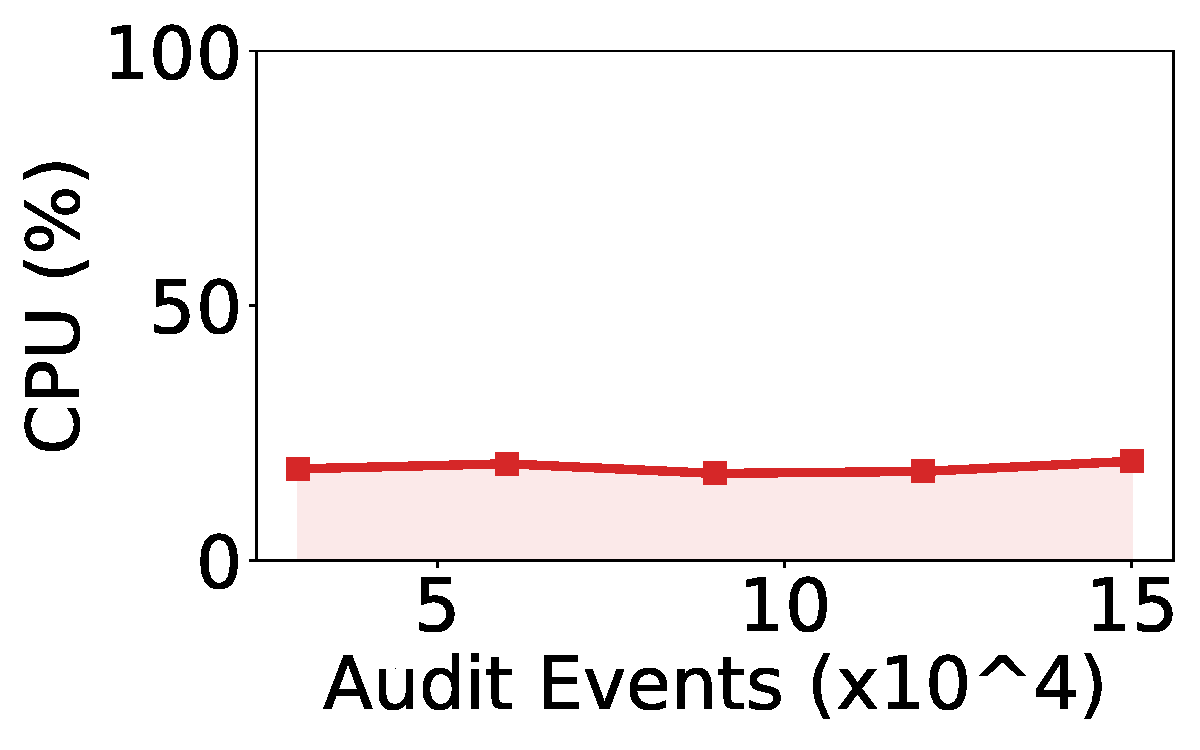
\includegraphics[width=0.20\textwidth]{fig/cpu.pdf}\label{cpu_client}}
%   \hfill
%   \subfloat[RAM utilization client side]{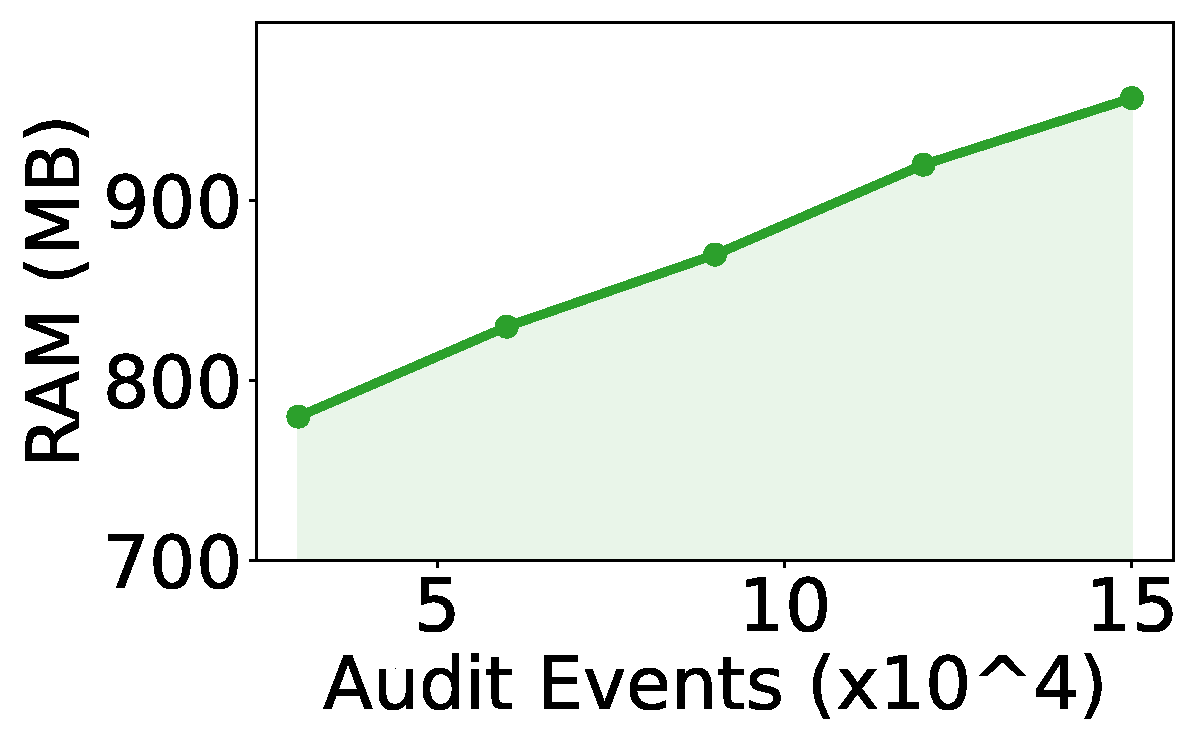
\includegraphics[width=0.20\textwidth]{fig/ram.pdf}\label{ram_client}}
%   \hfill
%   \subfloat[CPU utilization central server.]{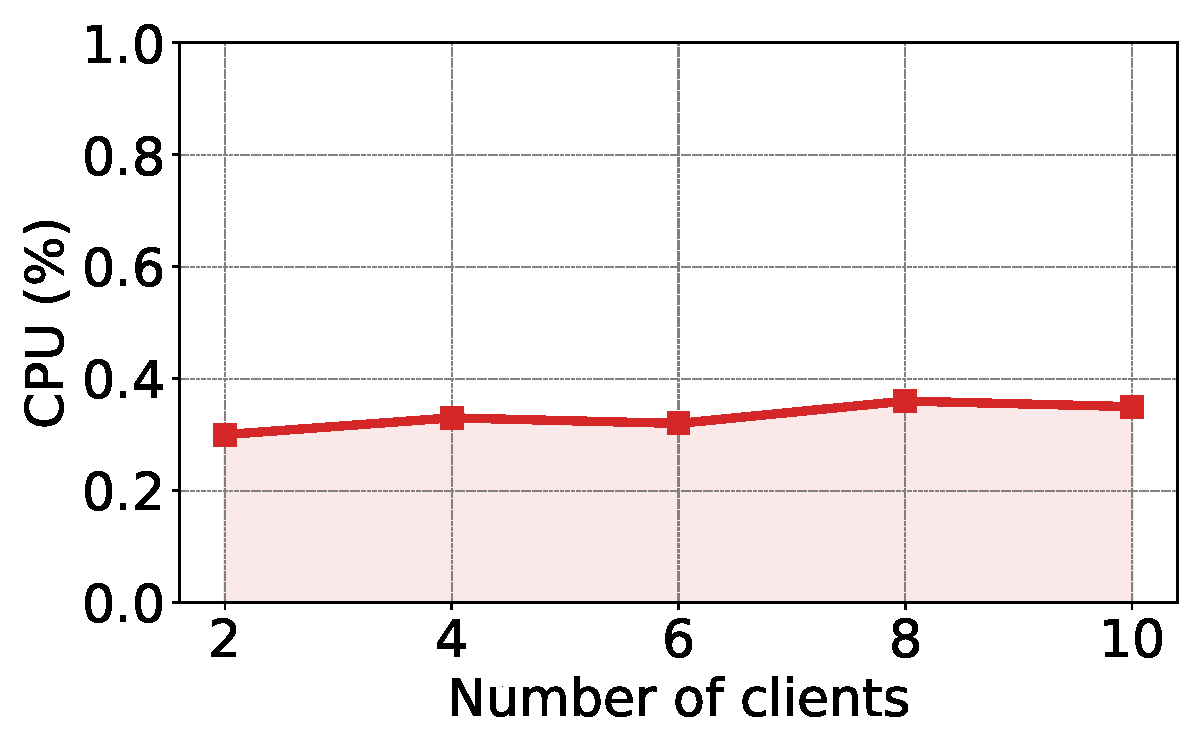
\includegraphics[width=0.20\textwidth]{fig/cpu_central.pdf}\label{cpu_central}}
%   \hfill
%   \subfloat[RAM utilization central server]{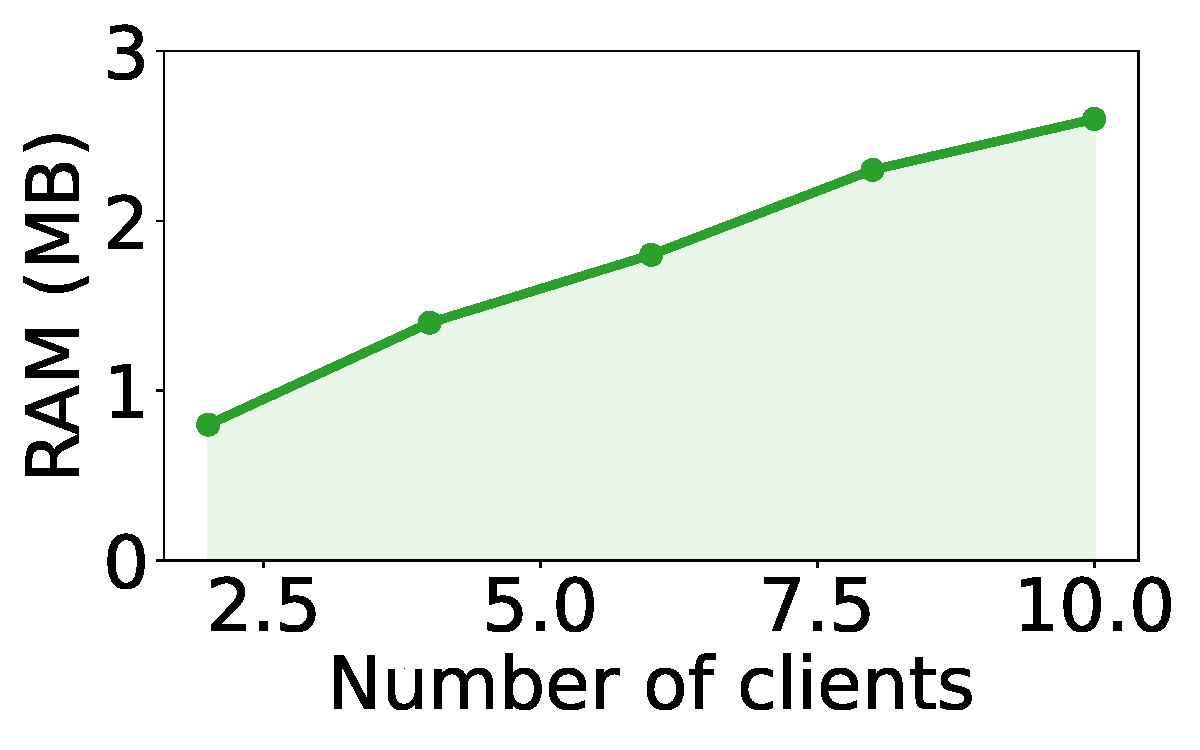
\includegraphics[width=0.20\textwidth]{fig/ram_central.pdf}\label{ram_central}}
%   \hfill
%   \subfloat[CPU utilization utility server.]{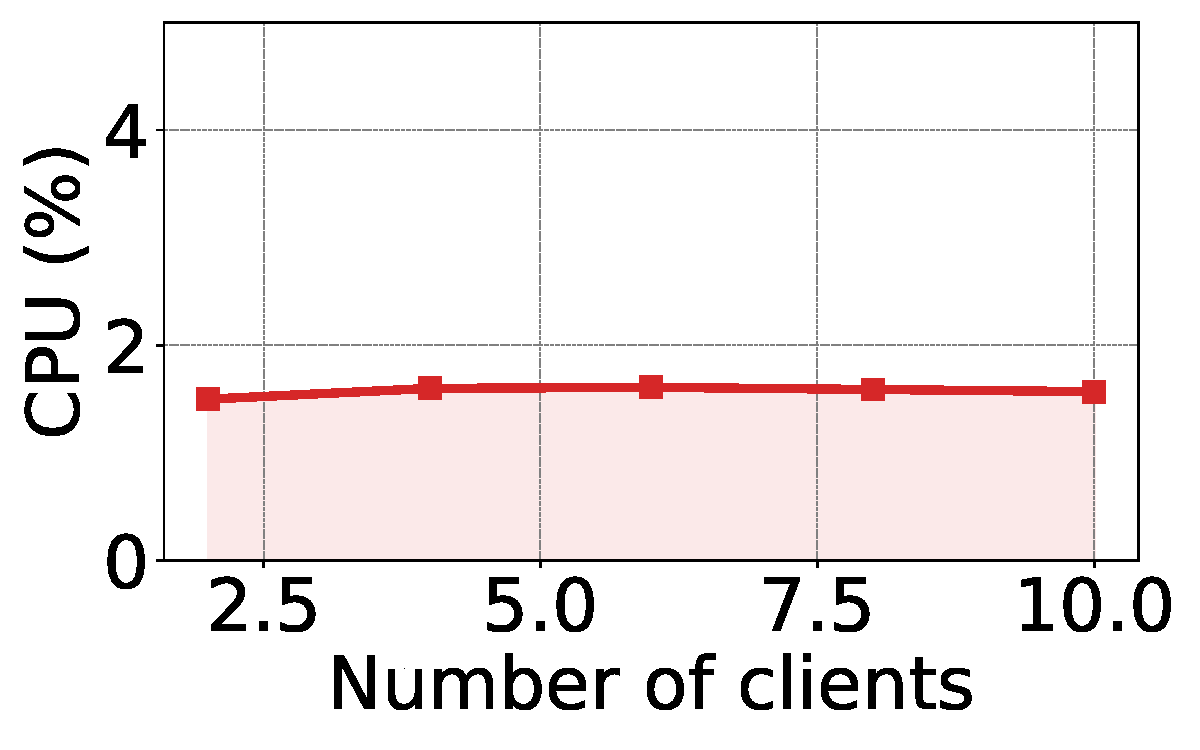
\includegraphics[width=0.20\textwidth]{fig/cpu_utility.pdf}\label{cpu_utility}}
%   \hfill
%   \subfloat[RAM utilization utility server]{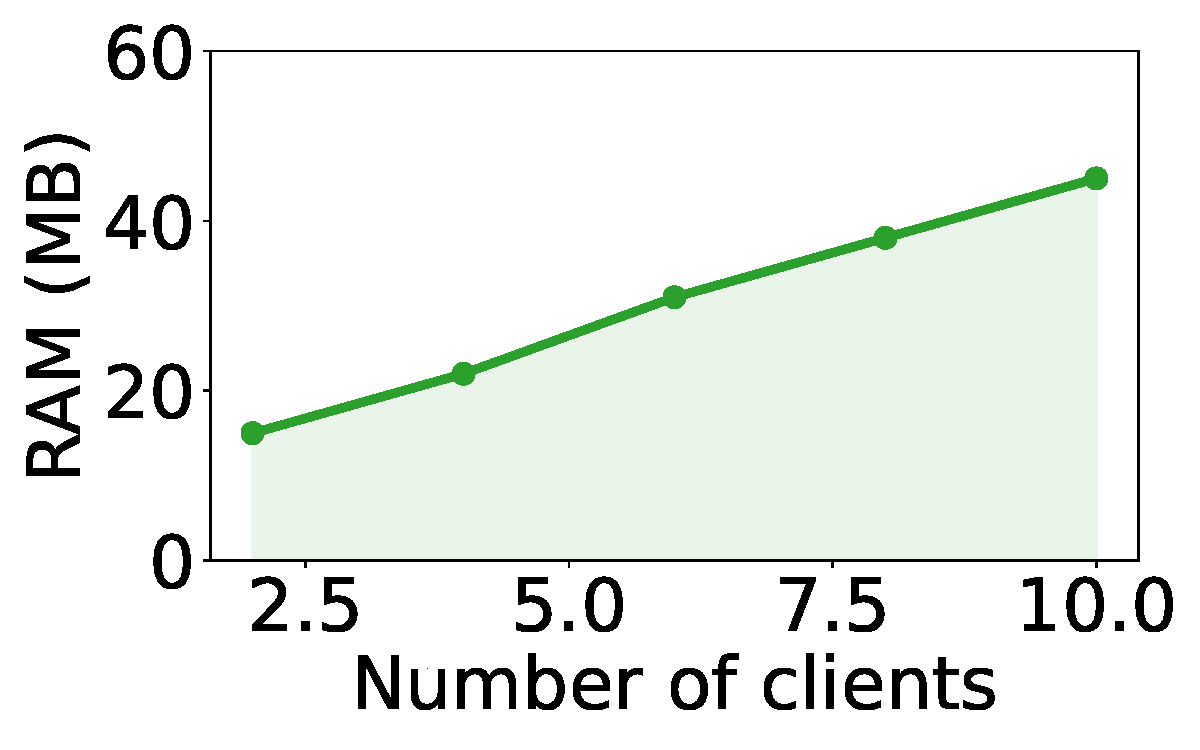
\includegraphics[width=0.20\textwidth]{fig/ram_utility.pdf}\label{ram_utility}}
%   \caption{Resource consumption of various components of \Sys.}
%   \label{fig:resource}
%   \vspace{-2ex}
% \end{figure}



% \subsection{Enterprise settings evaluation}
% \label{cost_metric}
% We examined the operational costs of deploying \Sys in comparison to centralized solutions like \flash and \kairos for organizational use. Our evaluation concentrates on two primary cost components: network expenses (\(C_{N}\)), and processing costs (\(C_{P}\)).

% \PP{Network Overhead:} We estimate this cost for the \flash and \kairos system using the \optc dataset. Each host within \optc produces approximately 1GB of audit logs daily, equating to nearly one million audit events. For an organization with 1,000 hosts, the total daily log volume would be 1,000 GB. This data volume necessitates transmission over the network to a central server operating the \pids. In contrast, \Sys achieves a significant reduction in these overheads. The only network expenses for \Sys arise from the transmission of the \gnnshort and \wordvec models; the \gnnshort model is roughly 13kb, while the average \wordvec model is 6 MB. Thus, the communication cost with the central server would be 12.70 MB, and for the utility server, it would be 5.86 GB. Ultimately, \Sys results in a 170-fold decrease in communication costs compared to \flash and \kairos.

% \PP{Processing Overhead:} Additionally, \flash processes one million events in about 100 seconds, implying that processing events from 1,000 clients would necessitate approximately 27.7 hours. In contrast, \kairos processes 57,000 events in 11.6 seconds, leading to a processing time of 204 seconds for one million events. Consequently, processing data from 1,000 clients with \kairos would require around 56.6 hours. Compared to existing systems, \Sys processes client logs in a decentralized manner and the total processing time is bounded by the client with the most log data; it will only take approximately 3 minutes to run inference on the complete \optc dataset. The central and utility servers conduct a simple mean operation on the models, taking only a few seconds.

% \PP{Overall Operating costs:} To calculate the daily operational costs of running these systems for a specific organization, we utilized the Google Cloud Platform's (GCP) pricing calculator~\cite{gcp}. The cost to operate \flash under the previously mentioned workload is estimated at \$135, with computing expenses accounting for \$100 and network costs comprising \$35. Given its longer processing duration, the operational cost for \kairos would be twice that of \flash. Compared to these systems, the operational cost of \Sys for 1,000 client machines would be approximately \$10 per day, marking a 13-fold reduction compared to \flash and a 26-fold reduction compared to \kairos.

% Scalability concerns are addressed in this section

\subsection{RQ3: Scalability in Enterprise settings}
\label{cost_metric}
We analyzed the performance of our system in an enterprise setting using the \optc dataset, which includes a large number of host machines. We compared our system to centralized systems such as \flash and \kairos, focusing on important metrics including network and processing overhead. \Fix{We also provide further discussion on scaling FL to massive enterprise networks in Appendix~\ref{state:explosion}.}

\PP{Network Overhead:} We estimate this cost for the \flash and \kairos system using the \optc dataset. Each host within \optc produces approximately 1GB of audit logs daily, equating to nearly one million audit events. For an organization with 1,000 hosts, the total daily log volume would be 1,000 GB. This data volume necessitates transmission over the network to a central server operating the \pids. In contrast, \Sys achieves a significant reduction in these overheads. The only network expenses for \Sys arise from the transmission of the \gnnshort and \wordvec models; the \gnnshort model is roughly \modelsize, while the average \wordvec model is 6 MB. Thus, the communication cost with the central server would be 12.70 MB, and for the utility server, it would be 5.86 GB. Hence, the network latency of model communications in \Sys is minimal compared to centralized systems where the raw system logs need to be sent over the network. Ultimately, \Sys results in a 170-fold decrease in communication costs compared to centralized \pids.  

\PP{Processing Overhead:} Additionally, \flash processes one million events in about 100 seconds, implying that processing events from 1,000 clients would necessitate approximately 27.7 hours. In contrast, \kairos processes 57,000 events in 11.6 seconds, leading to a processing time of 204 seconds for one million events. Consequently, processing data from 1,000 clients with \kairos would require around 56.6 hours. Compared to existing systems, \Sys processes client logs in a decentralized manner and the total processing time is bounded by the client with the most log data; it will only take approximately 3 minutes to run inference on the complete \optc dataset. The central and utility servers conduct a simple mean operation on the models, taking only a few seconds.

% \subsection{Robustness against mimicry attacks}
% \label{sec:mimicry}

% We assessed the robustness of our system against the adversarial mimicry attack proposed by Goyal et al.~\cite{goyal2023sometimes} using the E3 dataset. The attack's objective is to generate embeddings for nodes in the attack graphs that are similar to those in the benign graph, thus evading detection. To achieve this, structures from benign nodes are integrated into the attack graph. Figure~\ref{mimicryattack} illustrates the experimental results, with the x-axis representing the number of benign structures added and the y-axis corresponding to anomaly scores for all attack nodes. The findings indicate that our detector maintains robustness against this attack; adding benign structures has minimal effect on the anomaly scores of the attack nodes. The superior robustness of \Sys can be attributed to our process-categorization-based ensemble \gnnshort architecture, wherein each model specializes in understanding the behavior of specific system entities. Thus, when the graph structure surrounding these entities changes, the models can easily detect these alterations.\footnote{In contrast, the \flash system relies on a downstream model using \gnnshort embeddings to detect malicious entities. Generalizing a single model across system entities can cause it to overlook critical details, making it vulnerable to mimicry attacks. As demonstrated by the authors, \flash initially experiences a drop in anomaly scores, increasing the likelihood of attack nodes evading detection, a vulnerability not present in our system.}

% \begin{figure}[!t]
%   \centering
%   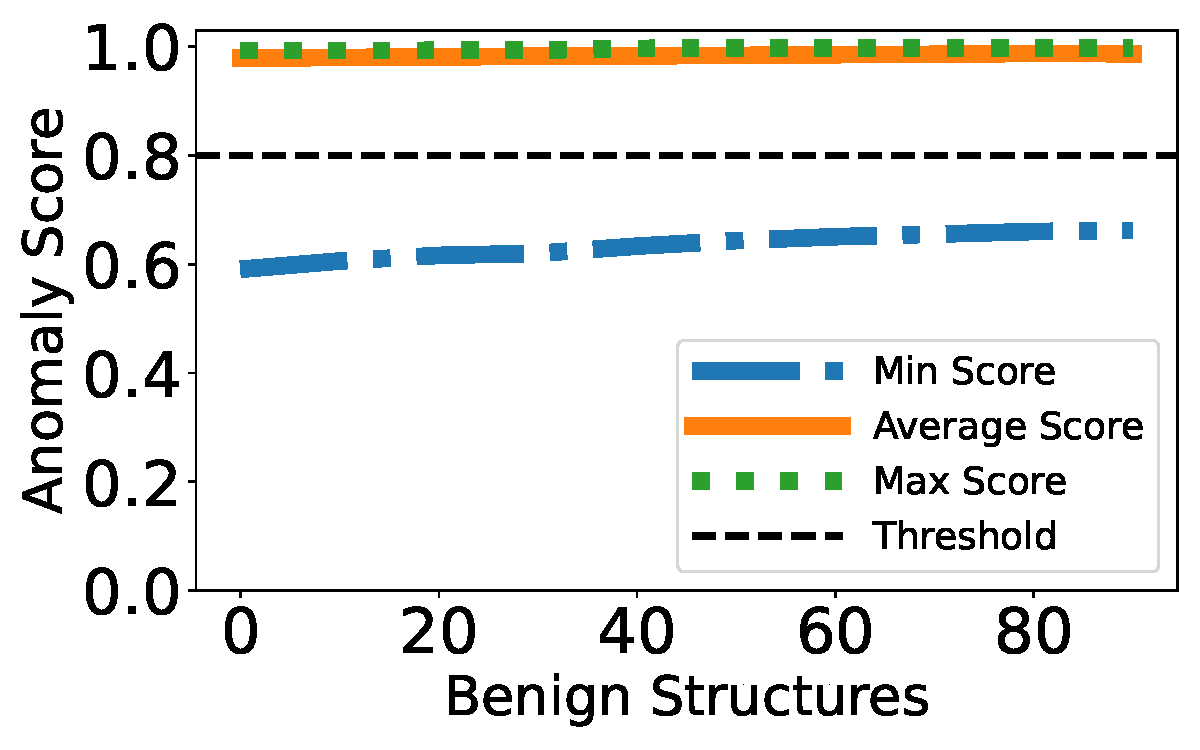
\includegraphics[width=0.4\textwidth]{fig/adversarial.pdf}
%   \caption{Adversarial mimicry attack analysis.}
%   \label{mimicryattack}
%   \vspace{-2ex}
% \end{figure}\


% \subsection{Effect of differential privacy on accuracy}

% Differential privacy is a method that can be combined with federated learning to offer protection against inference attacks~\cite{lyu2020threats,nasr2019comprehensive,zari2021efficient} at the cost of detection accuracy. We have analyzed the robustness of our system against these attacks in Section~\ref{privacy}. Here we will examine the impact of differential privacy noise levels on the detection performance of \Sys. Differential privacy achieves model privacy by adding a controlled amount of random noise to the model parameters, which helps in concealing the influence of any individual data point. In our context, differential privacy introduces a parameter called epsilon $\epsilon$ which dictates the intensity of noise added to the local \gnnshort model updates before they are aggregated at the central server for federated averaging, as detailed in Section~\ref{sec:methodology}.

% The parameter $\epsilon$ is crucial; it is inversely related to the amount of noise added -- lower values of $\epsilon$ result in higher noise levels, thereby increasing privacy but potentially degrading the utility of the model. Conversely, a higher $\epsilon$ indicates less noise, which may improve the model's detection capabilities but reduce privacy protection. By adjusting $\epsilon$ during the training phase, we assess the trade-off between privacy and detection performance in the globally trained models across various $\epsilon$ settings. Figure~\ref{epsvsscore} shows that increasing noise strength degrades model utility offering more privacy at the expense of reduced accuracy.

% \begin{figure}[!t]
%   \centering
%   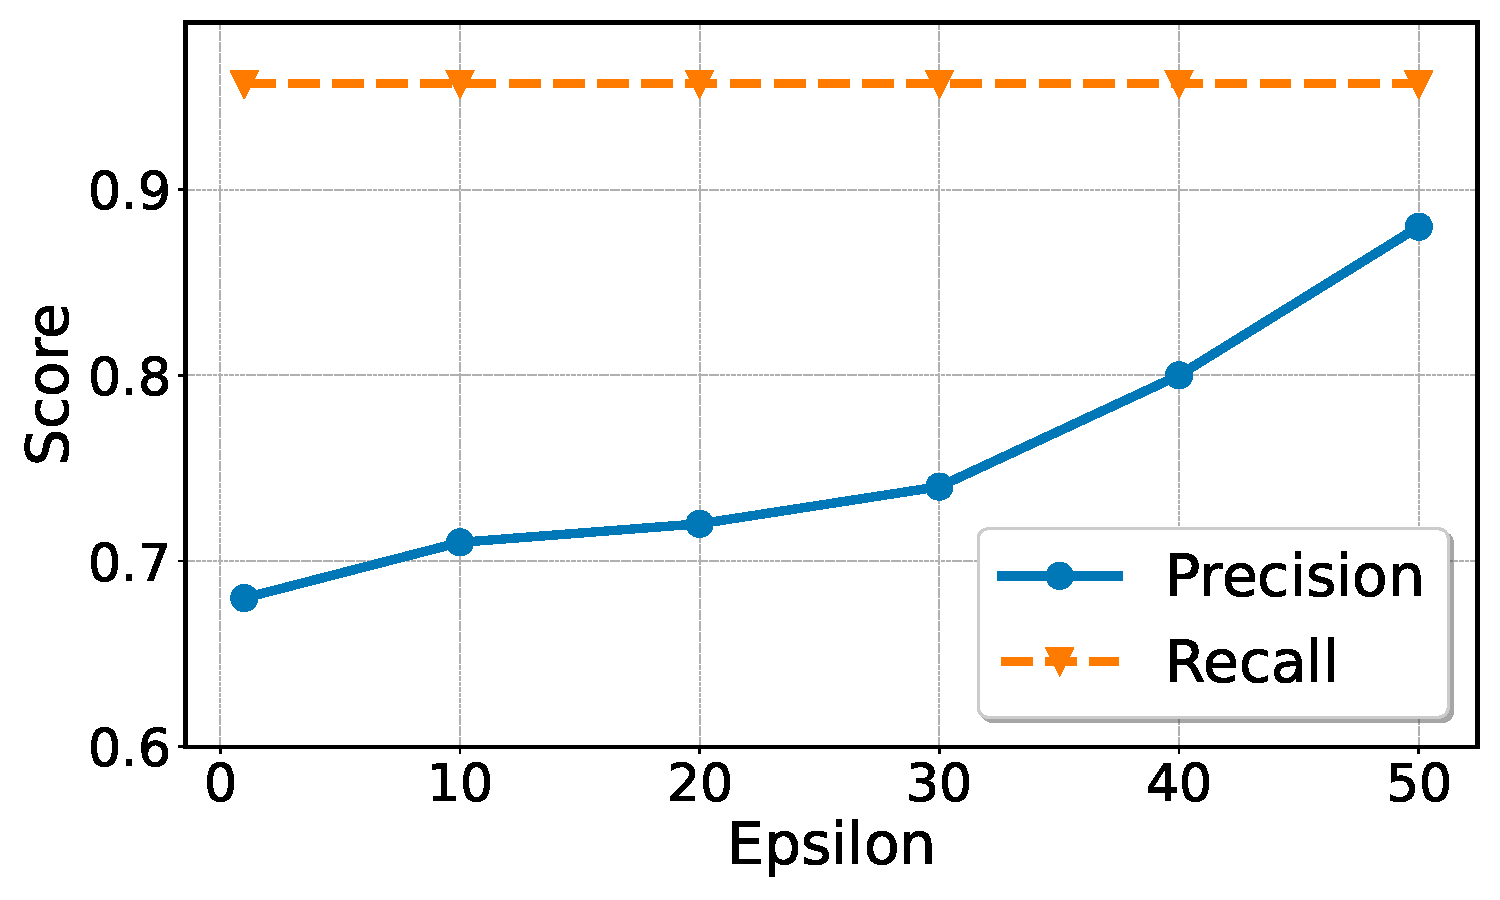
\includegraphics[width=0.25\textwidth]{fig/epsvsscore.pdf}
%   \caption{Effect of differential privacy noise on detection using E3 dataset. Note that we observed similar results on the other datasets.}
%   \label{epsvsscore}
%   \vspace{-2ex}
% \end{figure}


% \begin{figure*}[!t]
%   \centering
%   \subfloat[Anomaly threshold effect.]{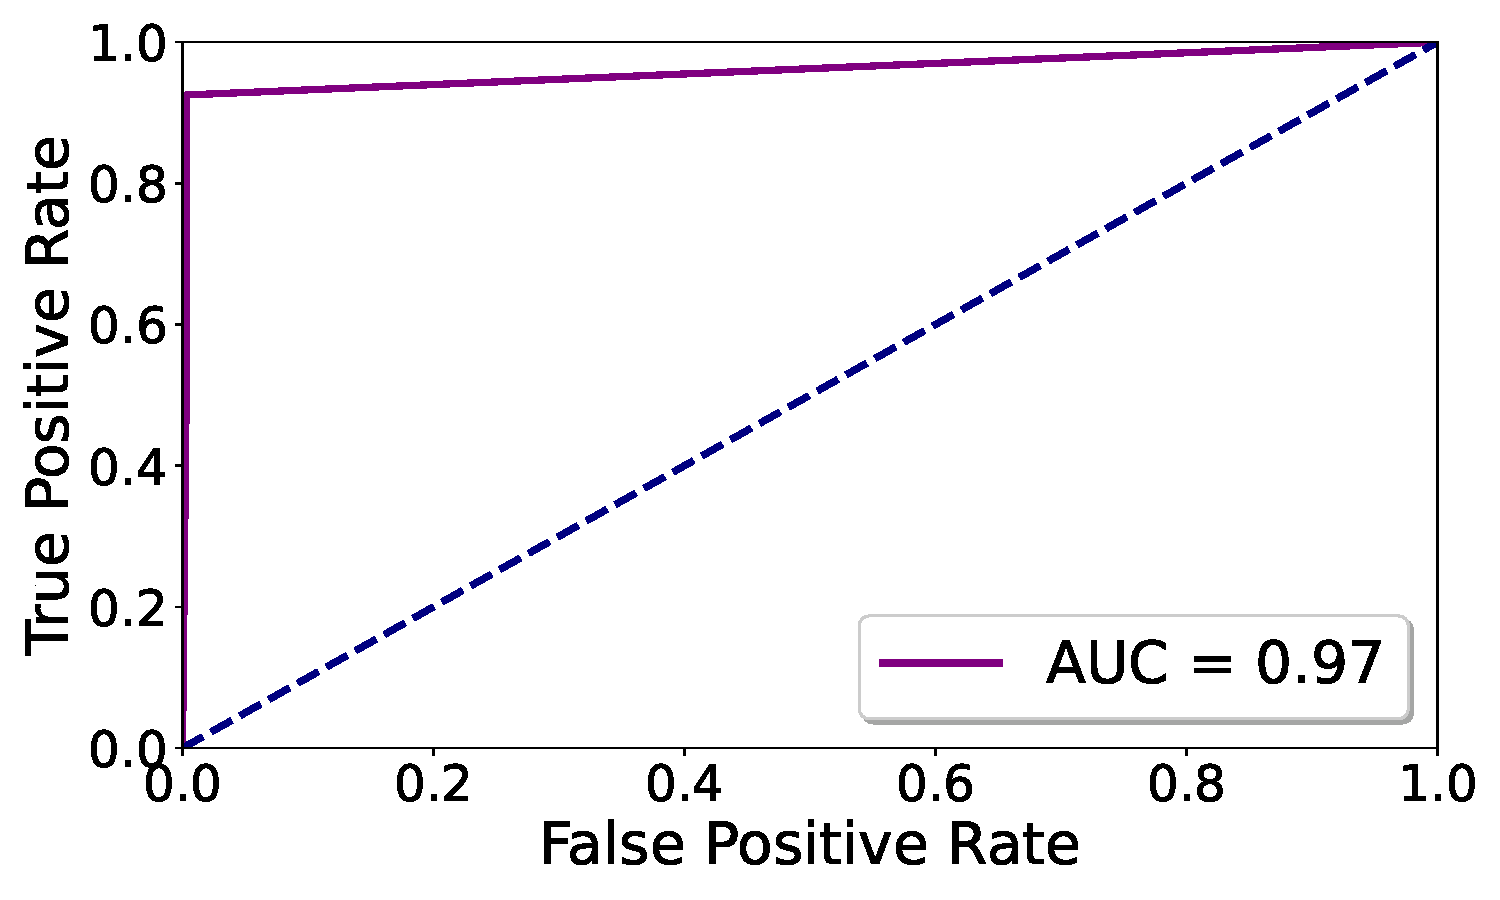
\includegraphics[width=0.24\textwidth]{fig/thresh.pdf}\label{thresh}}
%   \hfill
%   \subfloat[Effect of number of categories vs detection performance using E3 dataset.]{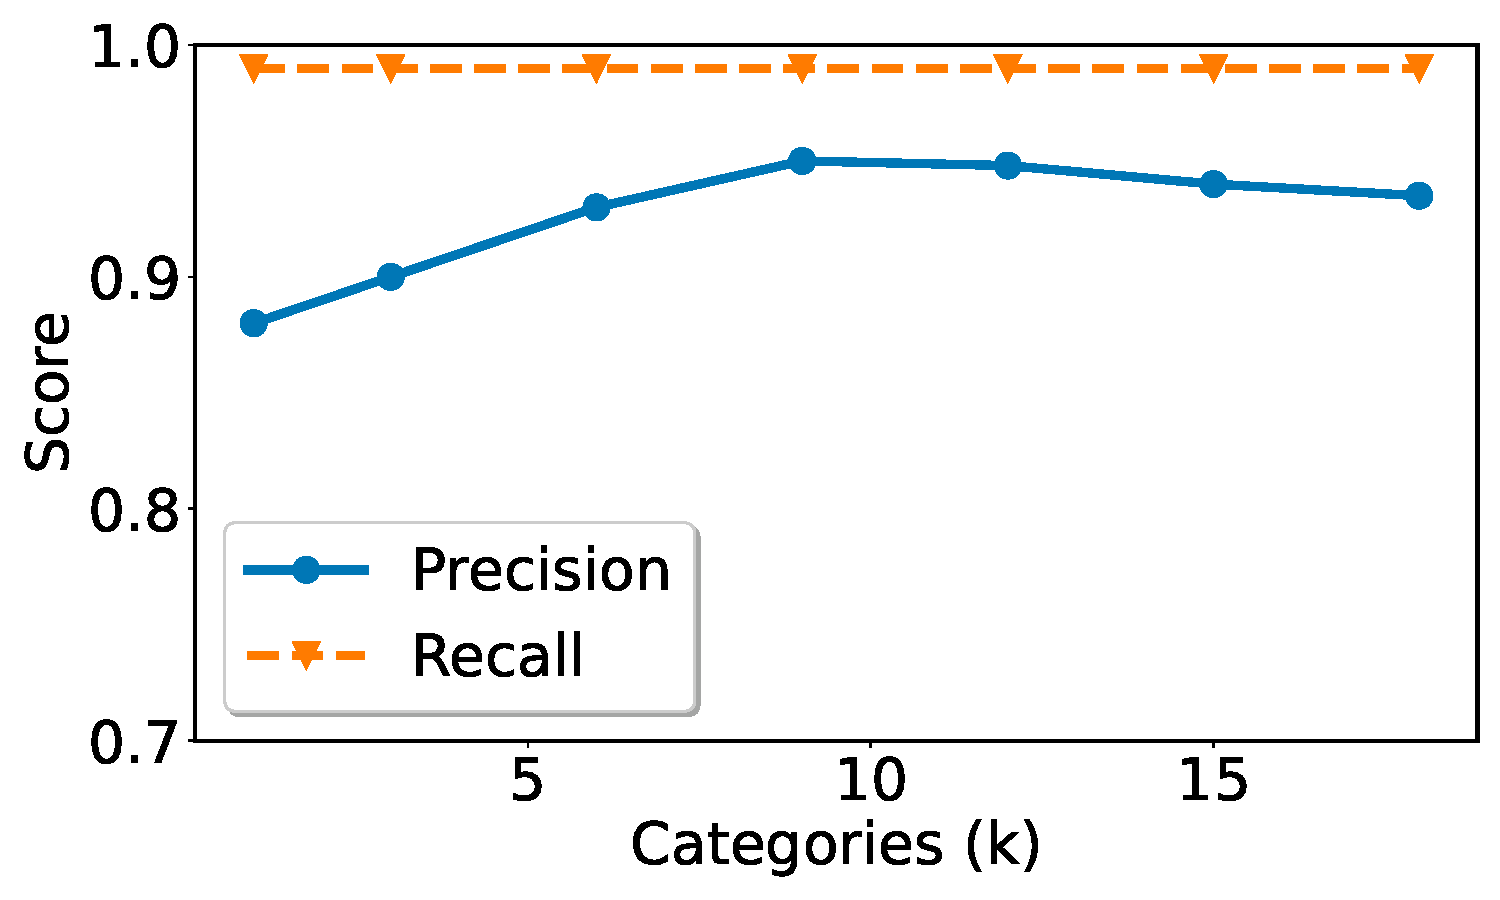
\includegraphics[width=0.24\textwidth]{fig/kvsscore.pdf}\label{catgvsscore}}
%   \hfill
%   \subfloat[Federated averaging rounds vs detection performance using E3 dataset.]{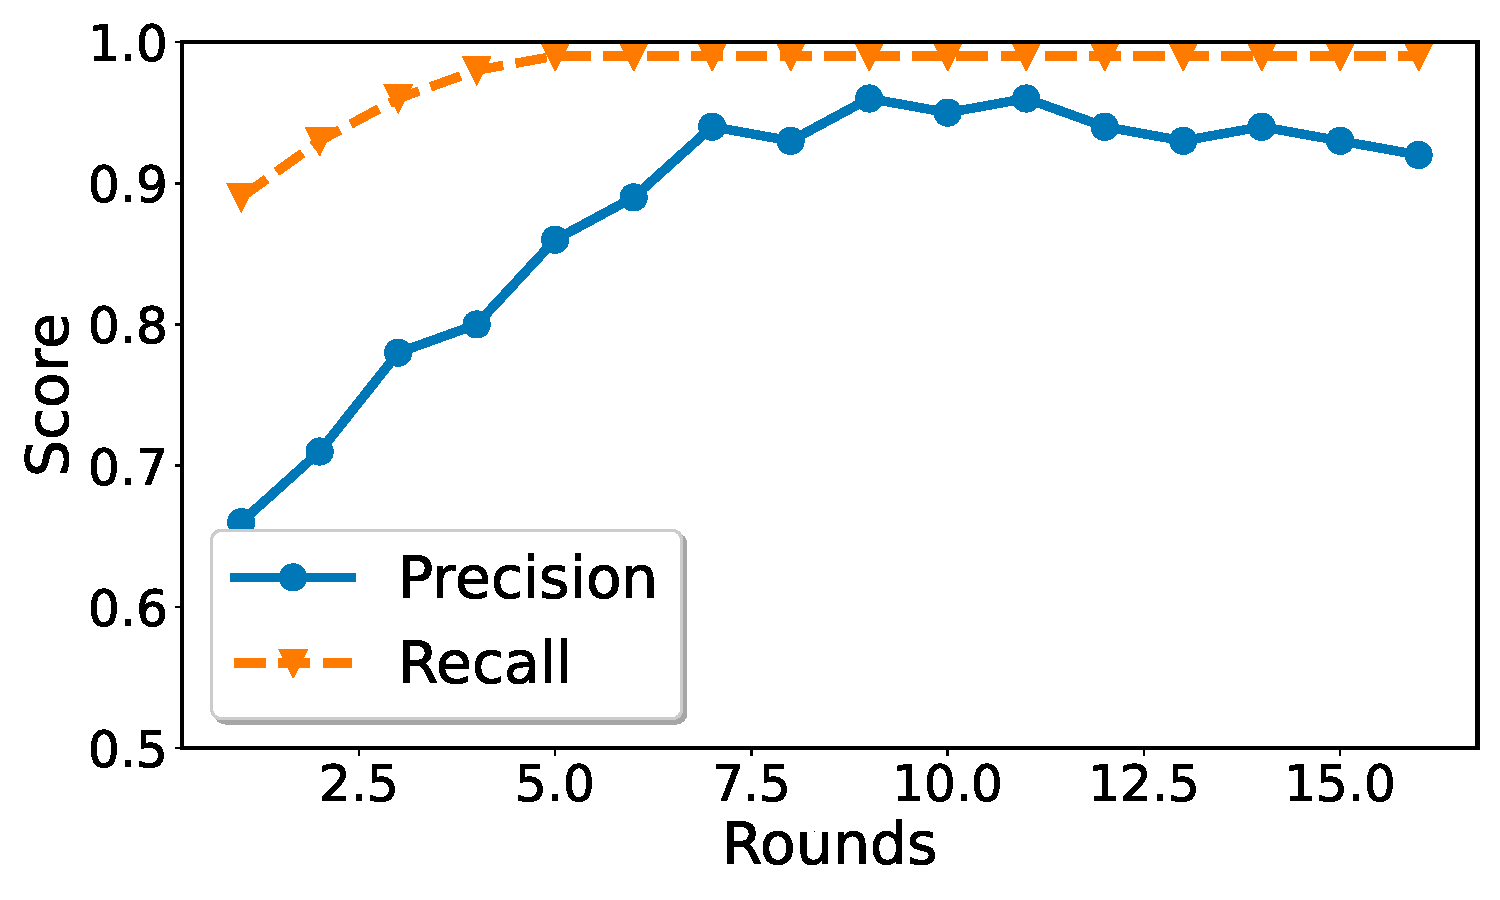
\includegraphics[width=0.24\textwidth]{fig/roundsvsscore.pdf}\label{roundsvsscore}}
%   \hfill
%   \subfloat[Effect of number of hosts vs detection metrics using \optc dataset]{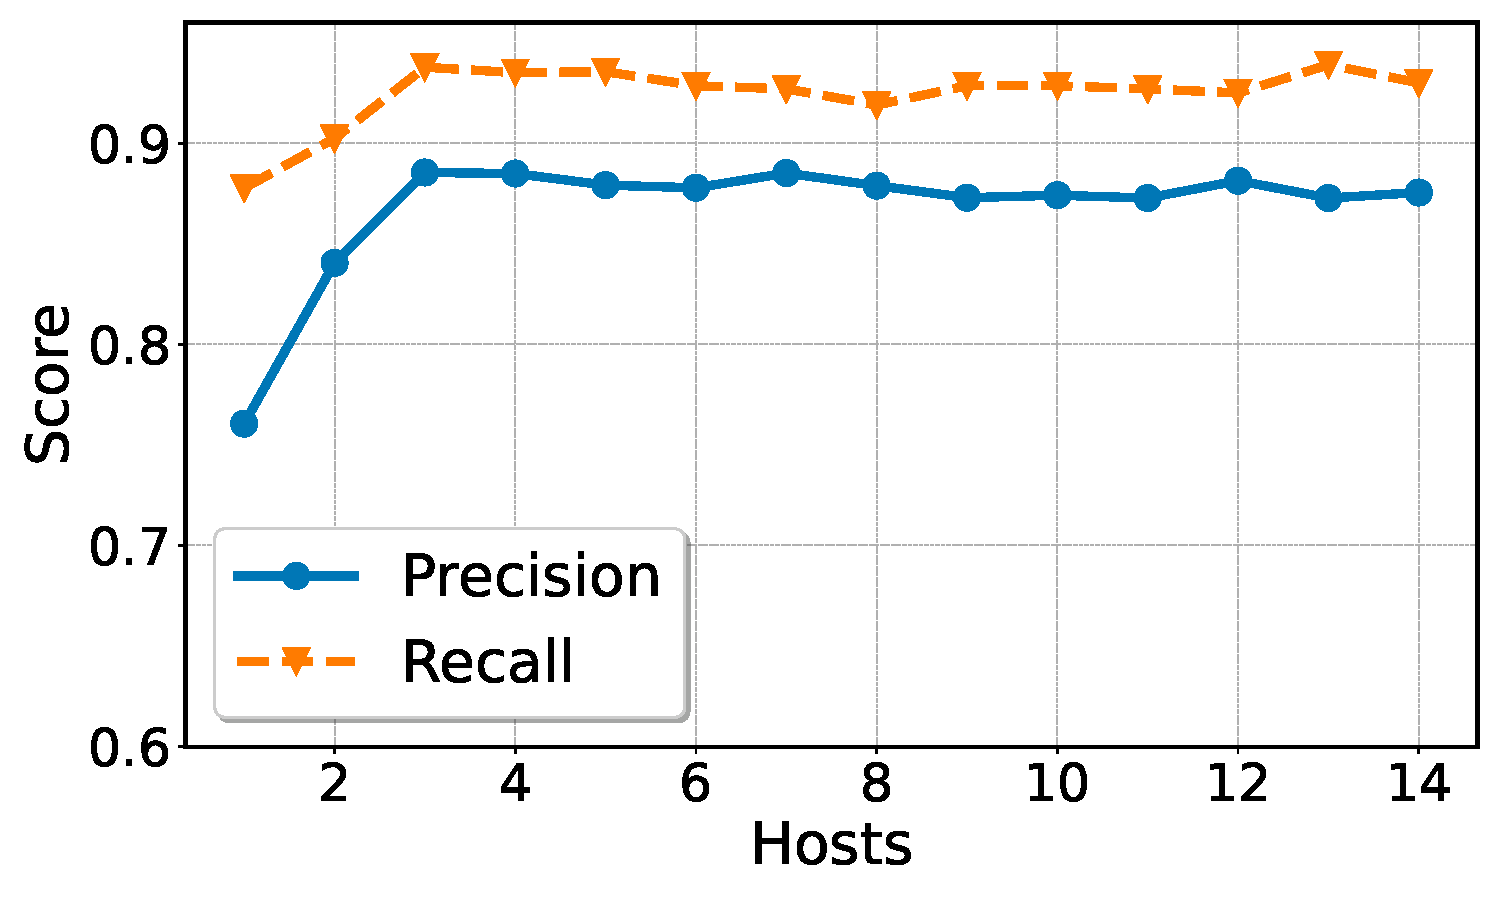
\includegraphics[width=0.24\textwidth]{fig/scoresvshosts.pdf}\label{rscoresvshosts}}
%   \caption{Ablation Study of various \Sys components.}
%   \label{ablation}
%   \vspace{-2ex}
% \end{figure*}
